% Springer LLNCS format — EAI INISCOM 2027 Submission
\documentclass[runningheads]{llncs}

\usepackage{graphicx}
\usepackage{float}
\usepackage{amsmath,amssymb,amsfonts}
\usepackage{booktabs}
\usepackage{multirow}
\usepackage{url}
\usepackage{xcolor}

\graphicspath{
    {figures/}
    {figures/tram1/}
    {figures/tram2/}
    {figures/rcATT/}
}

\begin{document}

\title{Contextual Data Augmentation for Imbalanced Multi-Label Classification of MITRE ATT\&CK Techniques Using Domain-Adapted BERT}

\titlerunning{CDA for Imbalanced ATT\&CK Classification}

\author{Anonymous Author(s)}

\authorrunning{Anonymous et al.}

\institute{Institution withheld for double-blind review}

\maketitle

% ============================================================
\begin{abstract}
Automated mapping of Cyber Threat Intelligence~(CTI) reports to the MITRE ATT\&CK framework is critical for proactive cybersecurity operations. However, existing machine learning pipelines face four persistent challenges: severe class imbalance suppressing Macro-F1 on rare classes, a lack of contextual information in short-text annotations, semantic label overlap between behaviourally adjacent techniques, and vocabulary adaptation across domain corpora. To address these limitations, this paper proposes a unified, reproducible framework using a domain-adapted BERT model integrated with Contextual Data Augmentation~(CDA) and task-specific loss functions. We systematically evaluate our approach across three public benchmarks under a controlled protocol to enable direct cross-task comparison. On the single-label TRAM~1 sentence dataset (50 classes), class-weighted cross-entropy achieves a Micro-F1 score of 0.6818 and a Macro-F1 score of 0.6160 without data augmentation. On the multi-label TRAM~2 sentence dataset (50 classes), combining background-noise downsampling (1:1), contextual data augmentation for minority classes, and Focal Loss significantly improves performance, raising the test Micro-F1 from 0.3344 to 0.5847 and Macro-F1 from 0.2767 to 0.4826 (a +74.5\% relative gain), with an Exact Match Ratio of 0.6130; repeated trials confirm high stability (mean Micro-F1 of $0.5706 \pm 0.0025$). Conversely, on the document-level rcATT dataset (227 classes), we expose a critical architectural constraint: the fixed 256-token context window retains only 3.9\% of each report on average, yielding a Macro-F1 score of 0.0368 and demonstrating that standard short-context architectures are fundamentally mismatched for document-level threat mapping. Finally, cross-dataset error analysis identifies obfuscation vocabulary overlap (T1027~$\to$~T1140) as the dominant failure mode in sentence-level classification.

\keywords{Cyber Threat Intelligence \and MITRE ATT\&CK \and SecBERT \and Multi-Label Classification \and Contextual Data Augmentation \and Class Imbalance \and Natural Language Processing}
\end{abstract}

% ============================================================
\section{Introduction}

\subsection{Background}
Cyber Threat Intelligence~(CTI) enables security operations teams to proactively identify adversary behaviors, improve detection rules, and expedite incident response by transforming raw telemetry and unstructured threat reports into structured, actionable intelligence~\cite{sun2023cti}. The MITRE ATT\&CK framework~\cite{strom2018attack} provides a standardized taxonomy of Tactics, Techniques, and Procedures~(TTPs) that has become the foundational operational standard for cataloging adversarial behaviors.

Mapping unstructured CTI narratives to standardized ATT\&CK identifiers is operationally vital but remains predominantly manual, requiring substantial domain expertise and suffering from inter-annotator disagreement~\cite{li2024automated}. Recent advances in transformer-based pretrained language models~\cite{devlin2019bert} have stimulated research into automated mapping. Nevertheless, practical deployment continues to encounter significant barriers related to data quality, label distribution, and architectural fit.

\subsection{Research Gaps}
Based on a systematic review of the automated ATT\&CK mapping literature~\cite{li2024automated,orbinato2022automatic,albarrak2025acmapper,kim2022ttp}, this work is guided by three experimentally motivated research gaps:

\textbf{GAP~1 --- Severe Class Imbalance and Background Noise.} Public CTI datasets exhibit pronounced long-tail distributions: TRAM~1 exhibits a 171$\times$ frequency disparity between its most and least frequent techniques (Table~\ref{tab:datasets}), while TRAM~2 compounds this challenge with 78.8\% background-noise sentences carrying no label. Standard fine-tuning under such conditions yields acceptable global Micro-F1 but near-zero recall on rare classes~\cite{kim2022ttp,albarrak2025acmapper}. Simple random oversampling risks overfitting without introducing lexical diversity. \emph{This paper addresses GAP~1 by coupling background-noise downsampling, Contextual Data Augmentation~(CDA), and Focal Loss, achieving a +74.5\% relative Macro-F1 gain on TRAM~2 (Section~\ref{sec:experiments}).}

\textbf{GAP~2 --- Text Granularity and Architectural Mismatch.} Prior studies operate at two conflicting extremes. Sentence-level benchmarks (TRAM~1 and TRAM~2) average fewer than 9 words per sample, discarding surrounding narrative context necessary to disambiguate intent~\cite{orbinato2022automatic,husari2017ttpdrill}. Conversely, document-level corpora such as rcATT~\cite{legoy2020rcatt} average 2,829 words per report, vastly exceeding the standard 256-to-512 token limits of common BERT encoders and causing silent truncation. \emph{We address the document-level dimension of GAP~2 by providing the first quantified measurement of 256-token truncation on rcATT, demonstrating why short-context transformers fail in this regime (Section~\ref{sec:experiments}).}

\textbf{GAP~3 --- Semantic Label Overlap.} ATT\&CK techniques within the same tactical objective frequently share near-identical technical vocabularies~\cite{albarrak2025acmapper}. For instance, T1027 (Obfuscated Files or Information) and T1140 (Deobfuscate/Decode Files or Information) describe inverse operations using identical terminology (\emph{encoded, packed, encrypted}). Disambiguating these semantics remains an open challenge~\cite{li2024automated}. \emph{We address GAP~3 through granular False Positive / False Negative analysis demonstrating that T1027 overlap is the dominant error mode across both sentence benchmarks (Section~\ref{sec:error_analysis}).}

\subsection{Backbone Selection and Vocabulary Rationale}
General-domain language models such as vanilla BERT~\cite{devlin2019bert} are pre-trained on generic text (Wikipedia, BookCorpus) and lack specialized exposure to dense technical subwords common in security disclosures. Several domain-specialized encoders have emerged, including SecureBERT~\cite{aghaei2022securebert}, CySecBERT~\cite{bayer2022cybersecbert}, and SecBERT~\cite{jackaduma2020secbert}. 

In this work, we deploy the publicly available checkpoint \texttt{nlpaueb/sec-bert-base}~\cite{secbert2022}. Originally developed by Loukas et al.~\cite{secbert2022} for processing formal regulatory and financial filings, this checkpoint provides a stabilized domain-adapted vocabulary (30,000 subwords) trained on technical, non-conversational corporate disclosures. Our experimental findings surface an important conceptual insight: specialized cybersecurity vocabulary pre-training alone is not the sole determinant of classification success; rather, targeted structural interventions---specifically background downsampling, contextual augmentation, and calibrated focal loss---drive the dominant performance gains under severe class imbalance.

\subsection{Research Objectives and Contributions}
This study evaluates a unified fine-tuning and augmentation methodology across three diverse CTI datasets under a consistent protocol. Our core contributions are:
\begin{enumerate}
  \item \textbf{A Controlled Multi-Benchmark Framework:} We establish a reproducible cross-dataset evaluation across single-label sentence (TRAM~1), multi-label sentence (TRAM~2), and document-level multi-label (rcATT) corpora using a common encoder, enabling direct cross-task comparison.
  \item \textbf{An Effective Rebalancing Pipeline for Multi-Label CTI:} We demonstrate that integrating 1:1 background downsampling, minority-class Contextual Data Augmentation~(CDA), and Focal Loss yields a +74.5\% relative gain in Macro-F1 (0.2767 $\to$ 0.4826) on TRAM~2, validated across repeated independent runs ($0.5706 \pm 0.0025$ Micro-F1).
  \item \textbf{Quantified Evidence of Document Truncation Bottlenecks:} We provide precise measurements on rcATT (mean 2,829 words / 6,538 WordPiece tokens) revealing that a 256-token context window retains only 3.9\% of document content on average (99.5\% truncated), definitively establishing that low Macro-F1 (0.0368) stems from architectural context mismatch rather than optimization failure.
  \item \textbf{Systematic Failure-Mode Characterization:} We identify T1027 obfuscation vocabulary overlap as the primary source of false positives across sentence-level threat mapping tasks.
\end{enumerate}

% ============================================================
\section{Related Work}

\subsection{Automated ATT\&CK Mapping and TTP Extraction}
Initial efforts in automated CTI analysis utilized keyword matching, expert regex rules, and TF-IDF representations~\cite{husari2017ttpdrill}. Legoy~\cite{legoy2020rcatt} introduced the rcATT benchmark, applying multi-label TF-IDF classifiers over complete CTI reports to predict 12 tactical categories with a Macro-F1 of 0.62. The MITRE Engenuity Center subsequently released TRAM~\cite{mitre2023tram} to advance sentence-level technique mapping. Following BERT's introduction~\cite{devlin2019bert}, transformer fine-tuning demonstrated marked improvements over traditional machine learning baselines~\cite{li2024automated,orbinato2022automatic}.

\subsection{Domain-Specific Transformers in Cybersecurity}
To address technical jargon in CTI reports, domain-tailored models such as SecureBERT~\cite{aghaei2022securebert}, CySecBERT~\cite{bayer2022cybersecbert}, and ATT\&CK-BERT~\cite{baseldella2022attackbert} were introduced. Orbinato et al.~\cite{orbinato2022automatic} evaluated transformer variants for ATT\&CK classification, confirming that domain-adapted architectures generally achieve superior representation stability over open-domain BERT on technical text.

\subsection{Class Imbalance and Data Augmentation}
CTI datasets naturally suffer from extreme long-tail distributions because adversaries deploy common execution and defense evasion techniques far more frequently than rare discovery or impact methods. Kim and Kim~\cite{kim2022ttp} explored Easy Data Augmentation~(EDA)~\cite{wei2019eda} to enhance minority ATT\&CK technique recall. 

The most directly comparable prior investigation is AC\_MAPPER~\cite{albarrak2025acmapper}, which combined class-aware upsampling with synonym substitution on the TRAM Bootstrap corpus, reporting a Macro-F1 of 0.8975 on 50 classes. However, rule-based synonym replacement frequently introduces semantically incongruous substitutions in specialized technical contexts. In contrast, our approach adopts Contextual Data Augmentation~(CDA)~\cite{kobayashi2018contextual} via \texttt{nlpaug}~\cite{ma2019nlpaug}, which leverages masked language model predictions to generate contextually coherent substitutions, combined with Focal Loss~\cite{lin2017focal} to suppress overwhelming background gradients in multi-label settings.

% ============================================================
\section{Methodology}

\subsection{Datasets}
We systematically evaluate three public CTI benchmarks spanning different label structures and text granularities (Table~\ref{tab:datasets}):
\begin{itemize}
  \item \textbf{TRAM~1}~\cite{mitre2023tram}: Single-label sentence classification over 50 MITRE ATT\&CK techniques.
  \item \textbf{TRAM~2}~\cite{mitre2023tram}: Multi-label sentence classification over 50 techniques, dominated by 78.8\% unlabelled background-noise sentences.
  \item \textbf{rcATT}~\cite{legoy2020rcatt}: Full-length report classification with 227 heterogeneous labels (12 tactics and 215 techniques).
\end{itemize}

\begin{table}[t]
\caption{Dataset Statistics Across the Three Evaluated CTI Benchmarks}
\label{tab:datasets}
\setlength{\tabcolsep}{5pt}
\centering
\begin{tabular}{lrrr}
\toprule
Property & TRAM~1 & TRAM~2 & rcATT \\
\midrule
Total samples (raw)           & 5,089       & 19,178      & 1,490 \\
Samples with $\geq$1 label    & 5,089       & 4,070       & 1,490 \\
Unique target labels          & 50          & 50          & 227   \\
Classification paradigm       & Single-label& Multi-label & Multi-label \\
Avg.\ text length (words)     & 8.7         & 8.9 (median 7) & 2,829 (median 1,733) \\
Most frequent label           & T1027 (685) & T1027 (678) & TA0005 (770) \\
Class imbalance ratio         & 171$\times$ & 97$\times$  & $>$100$\times$ \\
Background noise rate         & 0\%         & 78.8\%      & 0\% \\
\bottomrule
\end{tabular}
\end{table}

\begin{figure}[t]
  \centering
  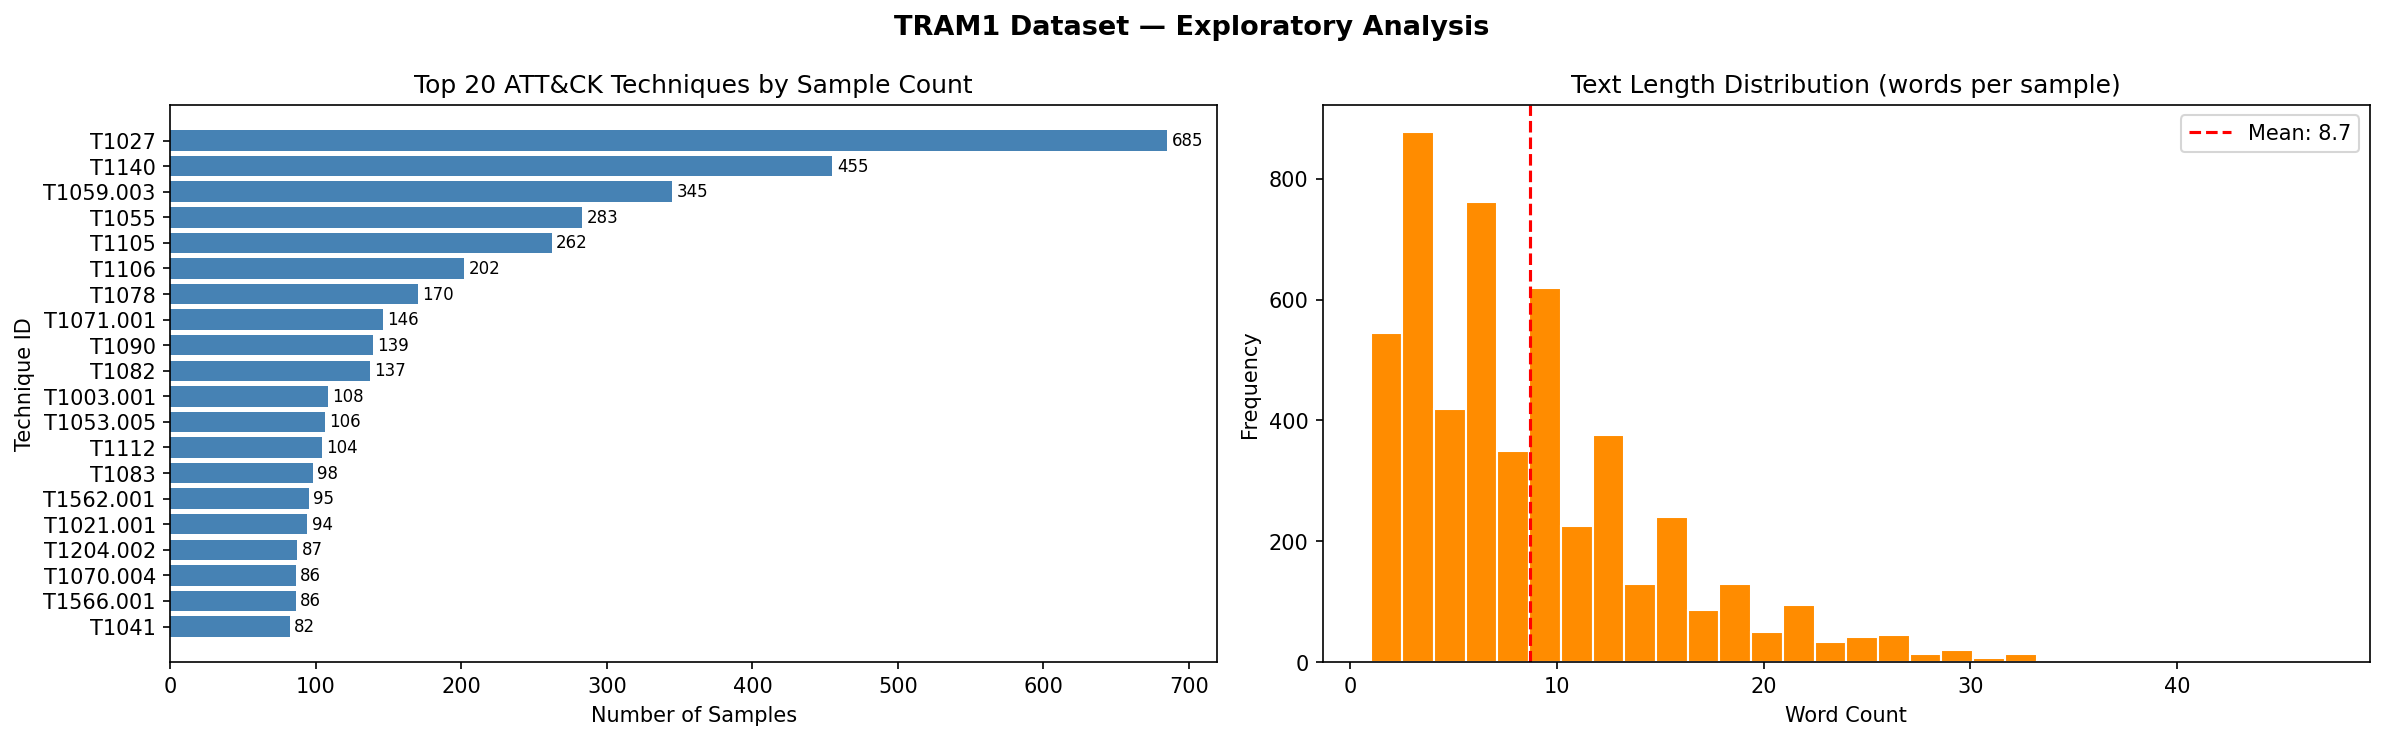
\includegraphics[width=\textwidth]{figures/tram1/tram1_cell2_eda.png}
  \caption{TRAM~1: (left) top-20 technique frequency; (right) text length distribution (mean 8.7 words). The 171$\times$ imbalance ratio and short text span represent key learning challenges.}
  \label{fig:tram1_eda}
\end{figure}

\begin{figure}[t]
  \centering
  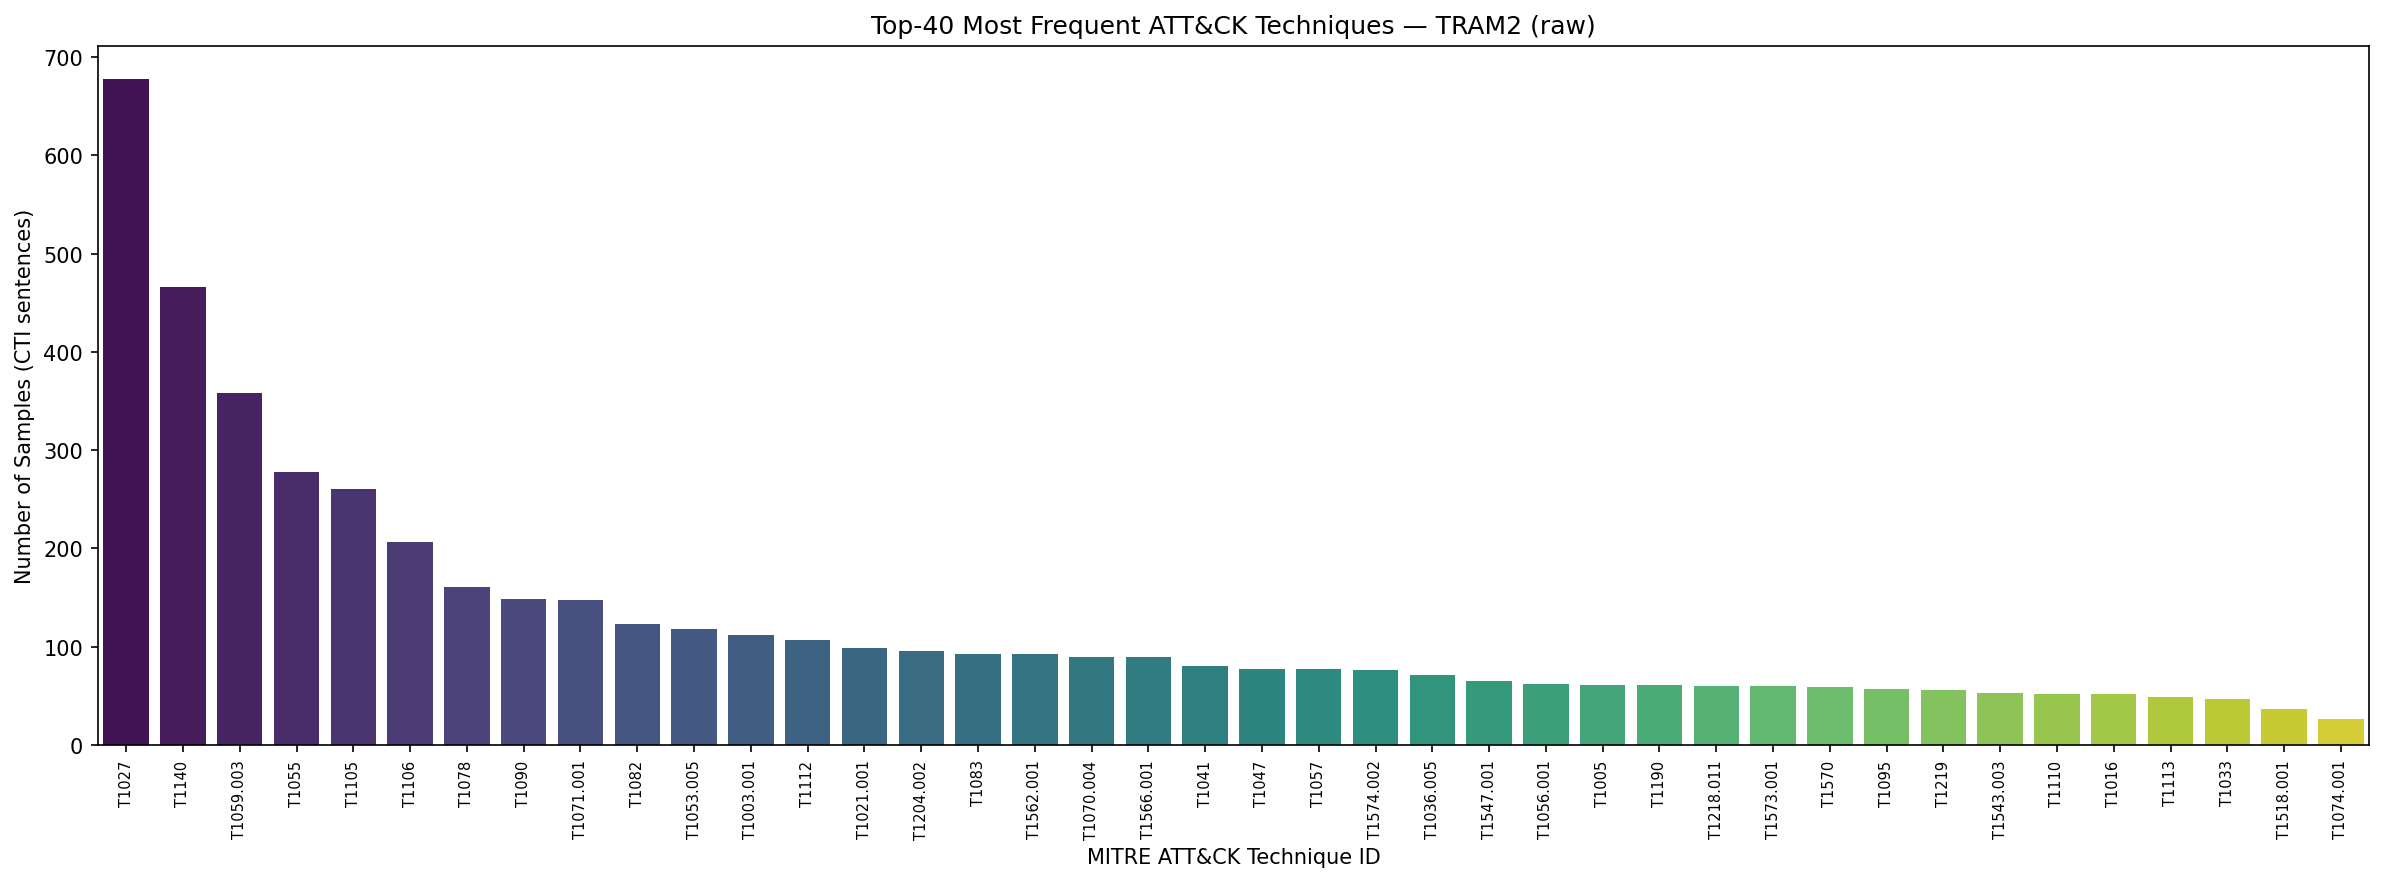
\includegraphics[width=\textwidth]{figures/tram2/tram2_tram2_cell2_eda_label_distribution.png}
  \caption{TRAM~2: top-40 technique frequency among labelled samples. 78.8\% of raw sentences contain no ATT\&CK labels (background noise).}
  \label{fig:tram2_eda}
\end{figure}

\subsection{Data Preprocessing and Augmentation}

\subsubsection{TRAM~1 (Single-Label Sentence).}
We first remove 252 exact-duplicate (text, label) pairs (4.9\%), leaving 4,837 distinct samples. The dataset is partitioned via stratified sampling (80\% train: 3,869; 10\% val: 484; 10\% test: 484). To counteract the 171$\times$ class imbalance without synthetically inflating the training set, we calculate inverse class frequencies~\cite{sklearn2011}:
\begin{equation}
  w_c = \frac{N}{K \cdot n_c}
  \label{eq:cw}
\end{equation}
where $N=3,869$ is the training size, $K=50$ is the number of classes, and $n_c$ is the frequency of class $c$.

\subsubsection{TRAM~2 (Multi-Label Sentence).}
The raw corpus contains 4,070 sentences with $\geq$1 ATT\&CK label and 15,108 unlabelled background sentences. Training directly on this raw distribution causes standard classifiers to collapse toward predicting empty sets. We downsample the unlabelled pool at a 1:1 ratio with labelled sentences, creating an 8,140-sentence working corpus. 

We then apply iterative stratification~\cite{sechidis2011} to preserve multi-label co-occurrence across splits (Train: 6,513; Val: 814; Test: 814). To bolster underrepresented classes, CDA~\cite{kobayashi2018contextual} via \texttt{nlpaug}~\cite{ma2019nlpaug} is applied exclusively to the training split for the 24 techniques with fewer than 50 examples ($p=0.15$ substitution probability, top-$k=20$), generating 469 synthetic samples (resulting in 6,982 training instances).

For the baseline multi-label configuration (BCE loss), positive class weights are computed as:
\begin{equation}
  \mathrm{pw}_c = \min\!\left(\frac{n_c^{-}}{n_c^{+} + \varepsilon},\; 50\right)
  \label{eq:pw}
\end{equation}
where $n_c^{-}$ and $n_c^{+}$ are negative and positive counts in training, $\varepsilon=10^{-5}$, and weights are capped at 50 to prevent gradient instability.

\subsubsection{rcATT (Document-Level Multi-Label).}
We utilize the canonical 1,490-report dataset~\cite{legoy2020rcatt} across 227 labels, using an 80/10/10 iterative split (Train: 1,172; Val: 151; Test: 167). When tokenized with WordPiece, rcATT reports average 6,538 tokens (median 3,980). A standard 256-token context window preserves only 3.9\% of each document on average, truncating 99.5\% of the corpus.

\subsection{Model Architecture and Objectives}
All tasks fine-tune the \texttt{nlpaueb/sec-bert-base} backbone~\cite{secbert2022}: 12 transformer layers, 768 hidden dimensions, 12 attention heads, and 109M parameters. A task-specific linear classification head maps the pooled representation to $K$ output logits.

\textbf{TRAM~1}: Fine-tuned with weighted cross-entropy (Eq.~\ref{eq:cw}) and $\arg\max$ prediction:
\begin{equation}
  \mathcal{L}_{\mathrm{WCE}} = -\sum_{c=1}^K w_c \cdot y_c \log(\hat{p}_c)
\end{equation}

\textbf{TRAM~2 Baseline}: Trained with positive-weighted Binary Cross-Entropy (Eq.~\ref{eq:pw}) and standard threshold $\tau=0.50$:
\begin{equation}
  \mathcal{L}_{\mathrm{WBCE}} = -\frac{1}{K}\sum_{c=1}^K \left[ \mathrm{pw}_c \cdot y_c \log(\sigma(z_c)) + (1-y_c)\log(1-\sigma(z_c)) \right]
\end{equation}

\textbf{TRAM~2 Optimized \& rcATT}: Trained with multi-label Focal Loss~\cite{lin2017focal} to down-weight easy background negatives:
\begin{equation}
  \mathcal{L}_{\mathrm{Focal}} = -\frac{1}{K}\sum_{c=1}^K \left[ \alpha (1-p_c)^\gamma y_c \log(p_c) + (1-\alpha) p_c^\gamma (1-y_c)\log(1-p_c) \right]
\end{equation}
where $p_c = \sigma(z_c)$, focusing parameter $\gamma = 2.0$, balancing factor $\alpha = 0.25$, and tuned inference threshold $\tau = 0.35$.

\begin{table}[t]
\caption{Experimental Hyperparameter Configurations Across Datasets}
\label{tab:hp}
\centering
\begin{tabular}{llll}
\toprule
Hyperparameter & TRAM~1 & TRAM~2 & rcATT \\
\midrule
Backbone & \multicolumn{3}{c}{\texttt{nlpaueb/sec-bert-base}~\cite{secbert2022}} \\
Max sequence length & 128 & 256 & 256 \\
Batch size / Epochs & 32 / 5 & 32 / 5 & 32 / 5 \\
Optimizer / Learning rate & \multicolumn{3}{c}{AdamW, $\eta = 2\times 10^{-5}$, linear warmup} \\
Loss function & Weighted CE & Focal Loss ($\gamma{=}2$) & Focal Loss ($\gamma{=}2$) \\
Classification threshold ($\tau$) & $\arg\max$ & 0.35 & 0.35 \\
Augmentation & None & CDA ($p{=}0.15, k{=}20$) & None \\
\bottomrule
\end{tabular}
\end{table}

% ============================================================
\section{Experiments and Results}
\label{sec:experiments}

\subsection{Evaluation Metrics}
Following established literature~\cite{li2024automated,albarrak2025acmapper,tsoumakas2007multilabel}, we evaluate:
\begin{itemize}
  \item \textbf{Micro-F1}: Aggregate metric reflecting global true positive, false positive, and false negative counts.
  \item \textbf{Macro-F1}: Unweighted arithmetic mean of per-class F1-scores, serving as the primary benchmark for imbalance robustness.
  \item \textbf{Exact Match Ratio (EMR)}: Fraction of test samples where the predicted multi-label set matches ground truth exactly. (Note: in downsampled TRAM~2, ~50\% of test instances are background negatives; predicting an empty set correctly earns EMR for such samples).
\end{itemize}

\subsection{TRAM~1 Results (Single-Label)}
Table~\ref{tab:tram1_epochs} and Figure~\ref{fig:tram1_curve} report TRAM~1 training progression. Macro-F1 increases monotonically from 0.1208 to 0.6448 on validation, reaching 0.6160 on the test split (Table~\ref{tab:all_results}). This demonstrates that class-weighted cross-entropy effectively prevents majority-class dominance without synthetic augmentation.

\begin{table}[t]
\caption{TRAM~1 Per-Epoch Validation Metrics}
\label{tab:tram1_epochs}
\centering
\begin{tabular}{ccccc}
\toprule
Epoch & Train Loss & Val Loss & Micro-F1 & Macro-F1 \\
\midrule
1 & 3.849 & 3.595 & 0.1715 & 0.1208 \\
2 & 3.305 & 2.822 & 0.4773 & 0.4190 \\
3 & 2.460 & 2.205 & 0.6095 & 0.5510 \\
4 & 2.052 & 1.875 & 0.6674 & 0.6186 \\
5 & 1.782 & 1.771 & 0.6901 & 0.6448 \\
\bottomrule
\end{tabular}
\end{table}

\begin{figure}[t]
  \centering
  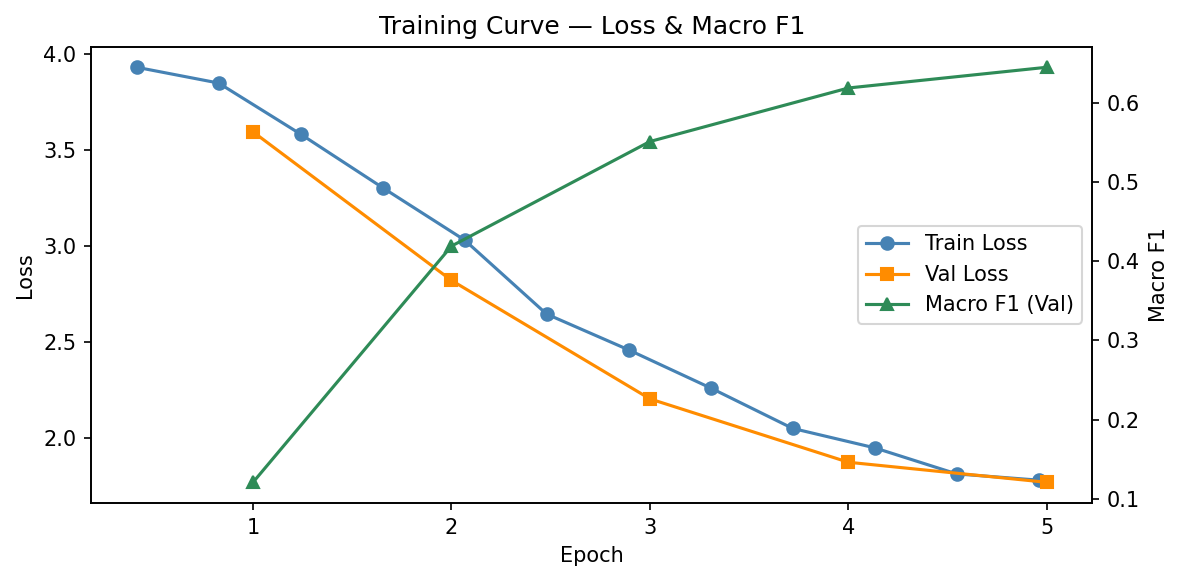
\includegraphics[width=0.88\textwidth]{figures/tram1/tram1_cell6_plot3_training_curve.png}
  \caption{TRAM~1 training curve over 5 epochs: loss (left) and validation Macro-F1 (right) demonstrate smooth convergence without overfitting.}
  \label{fig:tram1_curve}
\end{figure}

\subsection{TRAM~2 Results (Multi-Label)}
As shown in Table~\ref{tab:tram2_epochs} and Figure~\ref{fig:tram2_curve}, the optimized pipeline (Downsampling + CDA + Focal Loss) drives validation Macro-F1 from 0.0096 to 0.5628. On the independent 814-sentence test set, the optimized model achieves Micro-F1 = 0.5847, Macro-F1 = 0.4826, and EMR = 0.6130, outperforming the weighted BCE baseline by +0.2503 Micro-F1 and +0.2059 Macro-F1 (+74.5\% relative gain, Figure~\ref{fig:tram2_comp}).

\begin{table}[t]
\caption{TRAM~2 Optimized Configuration Per-Epoch Validation ($\tau = 0.35$)}
\label{tab:tram2_epochs}
\centering
\begin{tabular}{ccccc}
\toprule
Epoch & Train Loss & Micro-F1 & Macro-F1 & EMR \\
\midrule
1 & 0.0080 & 0.0479 & 0.0096 & 0.4988 \\
2 & 0.0048 & 0.2757 & 0.0477 & 0.5086 \\
3 & 0.0037 & 0.5046 & 0.2828 & 0.5676 \\
4 & 0.0027 & 0.5637 & 0.3648 & 0.6229 \\
5 & 0.0020 & 0.6105 & 0.5628 & 0.6130 \\
\bottomrule
\end{tabular}
\end{table}

\begin{figure}[t]
  \centering
  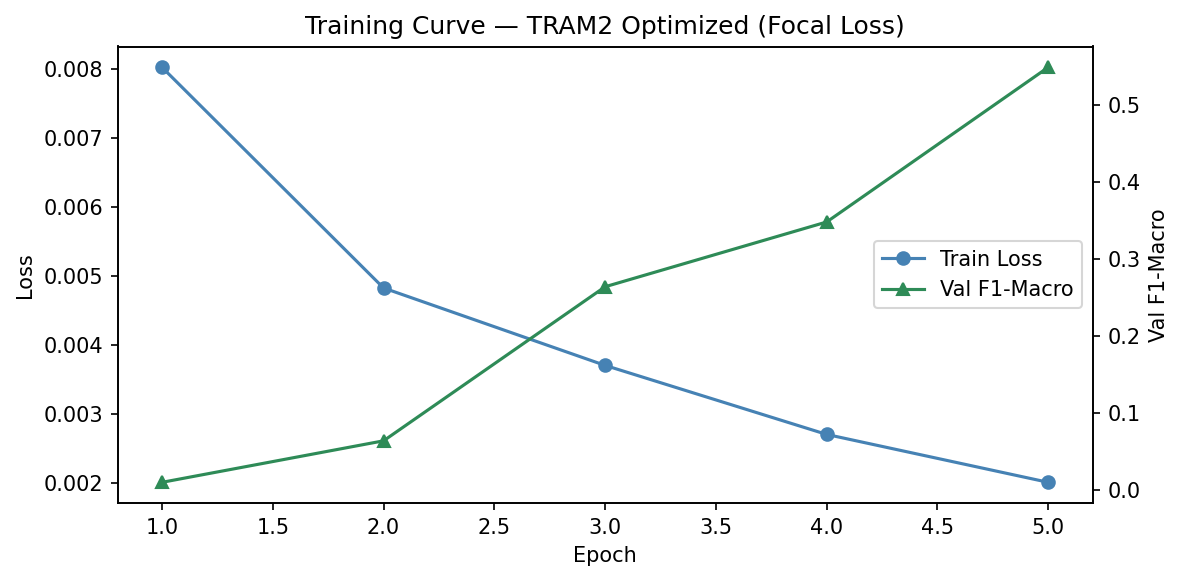
\includegraphics[width=0.88\textwidth]{figures/tram2/tram2_cell7_plot3_training_curve.png}
  \caption{TRAM~2 optimized model training trajectory: sharp gains in validation Macro-F1 occur from epoch 2 onward as Focal Loss suppresses background gradients.}
  \label{fig:tram2_curve}
\end{figure}

\begin{figure}[t]
  \centering
  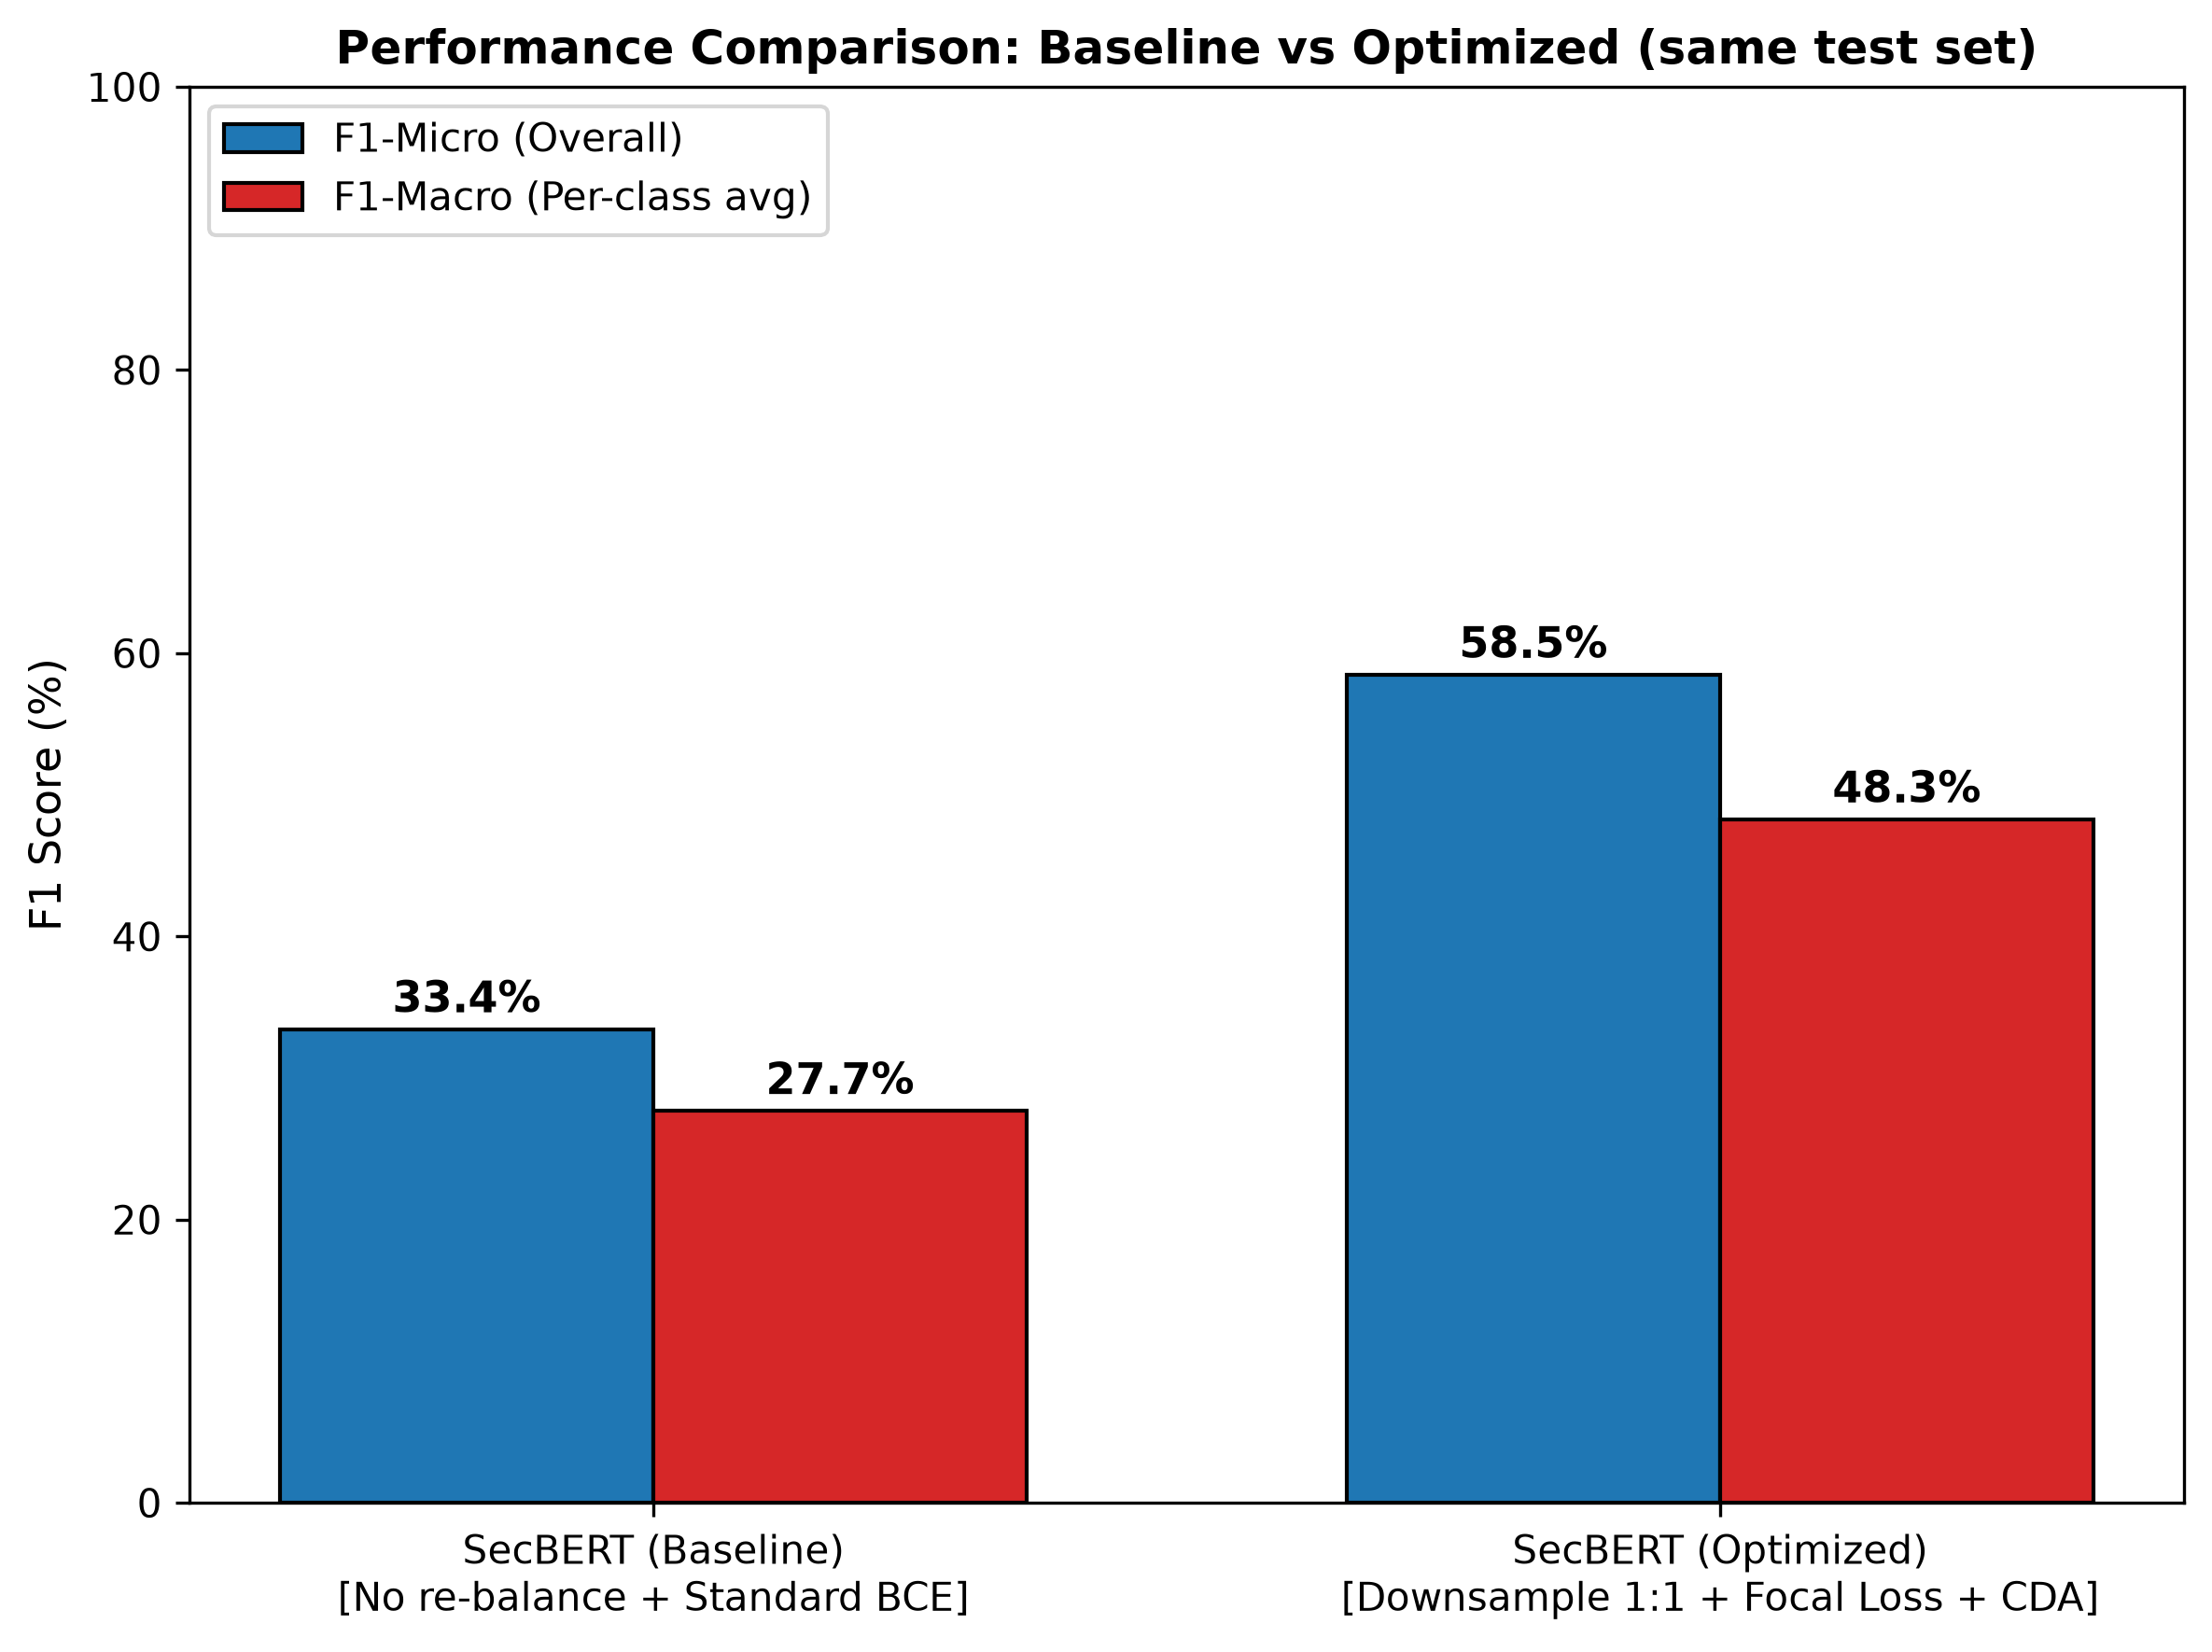
\includegraphics[width=0.82\textwidth]{figures/tram2/tram2_cell7_plot1_baseline_vs_optimized.png}
  \caption{Performance comparison on TRAM~2 test split between Baseline (weighted BCE, $\tau{=}0.5$) and Optimized (Downsample 1:1 + Focal Loss + CDA, $\tau{=}0.35$). Metrics show consistent gains across both overall Micro-F1 and per-class Macro-F1.}
  \label{fig:tram2_comp}
\end{figure}

\textbf{Cross-Run Stability.} To verify statistical reproducibility against seed sensitivity, we conducted four independent training runs on the identical test split. Across the four trials, the optimized configuration yielded remarkably tight bounds: test Micro-F1 of $0.5706 \pm 0.0025$ (range 0.5688--0.5735), Macro-F1 of $0.4666 \pm 0.0016$ (range 0.4647--0.4682), and EMR of $0.6057 \pm 0.0018$. In comparison, the baseline averaged Micro-F1 of $0.3224 \pm 0.0031$ and Macro-F1 of $0.2649 \pm 0.0028$. The consistent +74\% Macro-F1 margin confirms that performance gains stem from methodological design rather than stochastic variation.

\subsection{rcATT Results (Document-Level)}
On rcATT, the model achieves a test Micro-F1 of 0.0905 and Macro-F1 of 0.0368 with an EMR of 0.0000 (Figure~\ref{fig:rcatt_curve} and Table~\ref{tab:all_results}). While training loss decreases steadily, validation Macro-F1 oscillates near 0.04. 

This behavior is directly explained by the 256-token context bottleneck: rcATT reports average 6,538 WordPiece tokens, meaning 96.1\% of report tokens are silently omitted. Because crucial technical evidence is scattered throughout threat reports rather than concentrated in executive summaries, prefix truncation fatally impairs feature extraction. This confirms that short-context BERT encoders are architecturally mismatched for long-form threat analysis.

\begin{figure}[t]
  \centering
  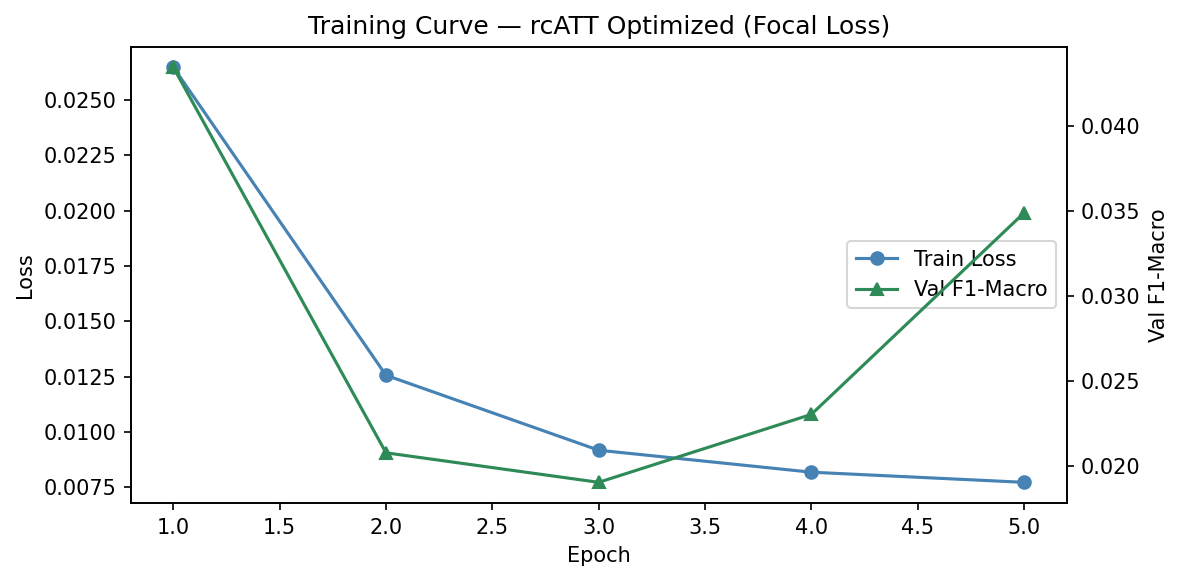
\includegraphics[width=0.88\textwidth]{figures/rcATT/rcATT_cell7_plot3_training_curve.png}
  \caption{rcATT training curve: loss decreases monotonically while validation Macro-F1 remains below 0.05, illustrating the severe architectural truncation constraint.}
  \label{fig:rcatt_curve}
\end{figure}

\subsection{Consolidated Benchmark Comparison}
Table~\ref{tab:all_results} summarizes our empirical results alongside pertinent prior publications.

\begin{table}[t]
\caption{Cross-Dataset Empirical Results and Comparison with Prior Literature}
\label{tab:all_results}
\setlength{\tabcolsep}{4.5pt}
\centering
\begin{tabular}{llcccc}
\toprule
Method & Benchmark & Classes & Micro-F1 & Macro-F1 & EMR \\
\midrule
\multicolumn{6}{l}{\textit{Prior Work}} \\
Legoy~\cite{legoy2020rcatt} (TF-IDF) & rcATT (tactics only) & 12 & --- & 0.6200 & --- \\
Orbinato et al.~\cite{orbinato2022automatic} (BERT) & CTI sentence corpus & 50 & 0.6500 & --- & --- \\
Kim \& Kim~\cite{kim2022ttp} (EDA) & Custom CTI corpus & --- & --- & $\uparrow$ vs base & --- \\
Li et al.~\cite{li2024automated} (BiLSTM+Attn) & Custom CTI reports & --- & 0.7200 & 0.6800 & --- \\
AC\_MAPPER~\cite{albarrak2025acmapper} (Upsampling+Syn) & TRAM Bootstrap$^\dagger$ & 50 & --- & 0.8975 & --- \\
\midrule
\multicolumn{6}{l}{\textit{This Work (\texttt{nlpaueb/sec-bert-base}, unified evaluation protocol)}} \\
Ours & TRAM~1 (Single-label) & 50 & 0.6818 & 0.6160 & 0.6818 \\
Ours (Baseline) & TRAM~2 (Multi-label) & 50 & 0.3344 & 0.2767 & 0.3821 \\
Ours (Optimized, best) & TRAM~2 (Multi-label) & 50 & \textbf{0.5847} & \textbf{0.4826} & \textbf{0.6130} \\
Ours (Optimized, 4-run mean) & TRAM~2 (Multi-label) & 50 & 0.5706 & 0.4666 & 0.6057 \\
Ours (Optimized) & rcATT (Document-level) & 227 & 0.0905 & 0.0368 & 0.0000 \\
\bottomrule
\multicolumn{6}{l}{\small $^\dagger$TRAM Bootstrap is a distinct curated subset; numbers are not directly comparable to TRAM~1/2.}
\end{tabular}
\end{table}

\textbf{Discussion of AC\_MAPPER:} AC\_MAPPER~\cite{albarrak2025acmapper} achieved a Macro-F1 of 0.8975 on the single-label TRAM Bootstrap dataset using synonym substitution. Crucially, TRAM Bootstrap is an artificially curated subset distinct from the raw, noisy TRAM~1 and TRAM~2 datasets evaluated here, precluding direct numerical equivalence. Furthermore, while AC\_MAPPER addressed only single-label classification, our framework systematically extends to multi-label sentence and full-document contexts.

% ============================================================
\section{Error Analysis}
\label{sec:error_analysis}

\subsection{TRAM~1: Confusion and Obfuscation Overlap}
Among 154 classification errors on the TRAM~1 test set ($154/484 \approx 31.8\%$), two confusion pairs dominate: T1027~$\to$~T1140 (23 instances) and T1027~$\to$~T1573.001 (18 instances), accounting for 26.6\% of all test errors (Figure~\ref{fig:tram1_errors}). T1027 (Obfuscated Files) and T1140 (Deobfuscate Files) represent inverse operational concepts described using identical keywords (\emph{encoded, decoded, XOR, base64}), confirming GAP~3.

\begin{figure}[t]
  \centering
  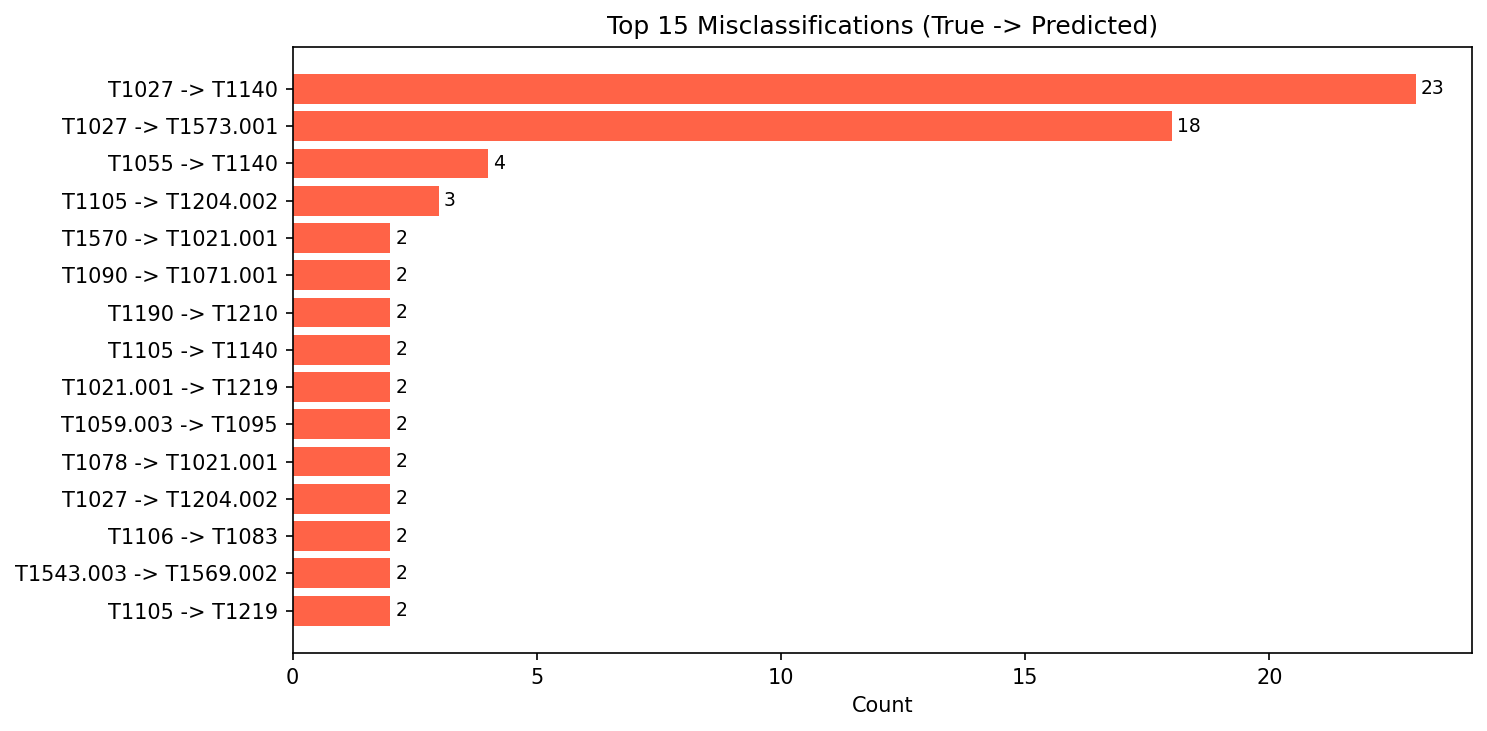
\includegraphics[width=\textwidth]{figures/tram1/tram1_cell7_plot2_top_errors.png}
  \caption{Top-15 misclassification pairs on TRAM~1. Shared obfuscation terminology between T1027 and T1140 accounts for the largest cluster of confusion.}
  \label{fig:tram1_errors}
\end{figure}

\subsection{TRAM~2: False Positive vs. False Negative Dynamics}
Figure~\ref{fig:tram2_errors} dissects the top-15 error-prone techniques in TRAM~2 into False Positives (FP) and False Negatives (FN). T1027 generates 48 FPs and 23 FNs (71 total errors), reinforcing that semantic overlap identified in TRAM~1 is magnified in multi-label scenarios where multiple techniques co-occur. Conversely, techniques with limited test support (T1012, T1518.001) primarily suffer from False Negatives.

\begin{figure}[t]
  \centering
  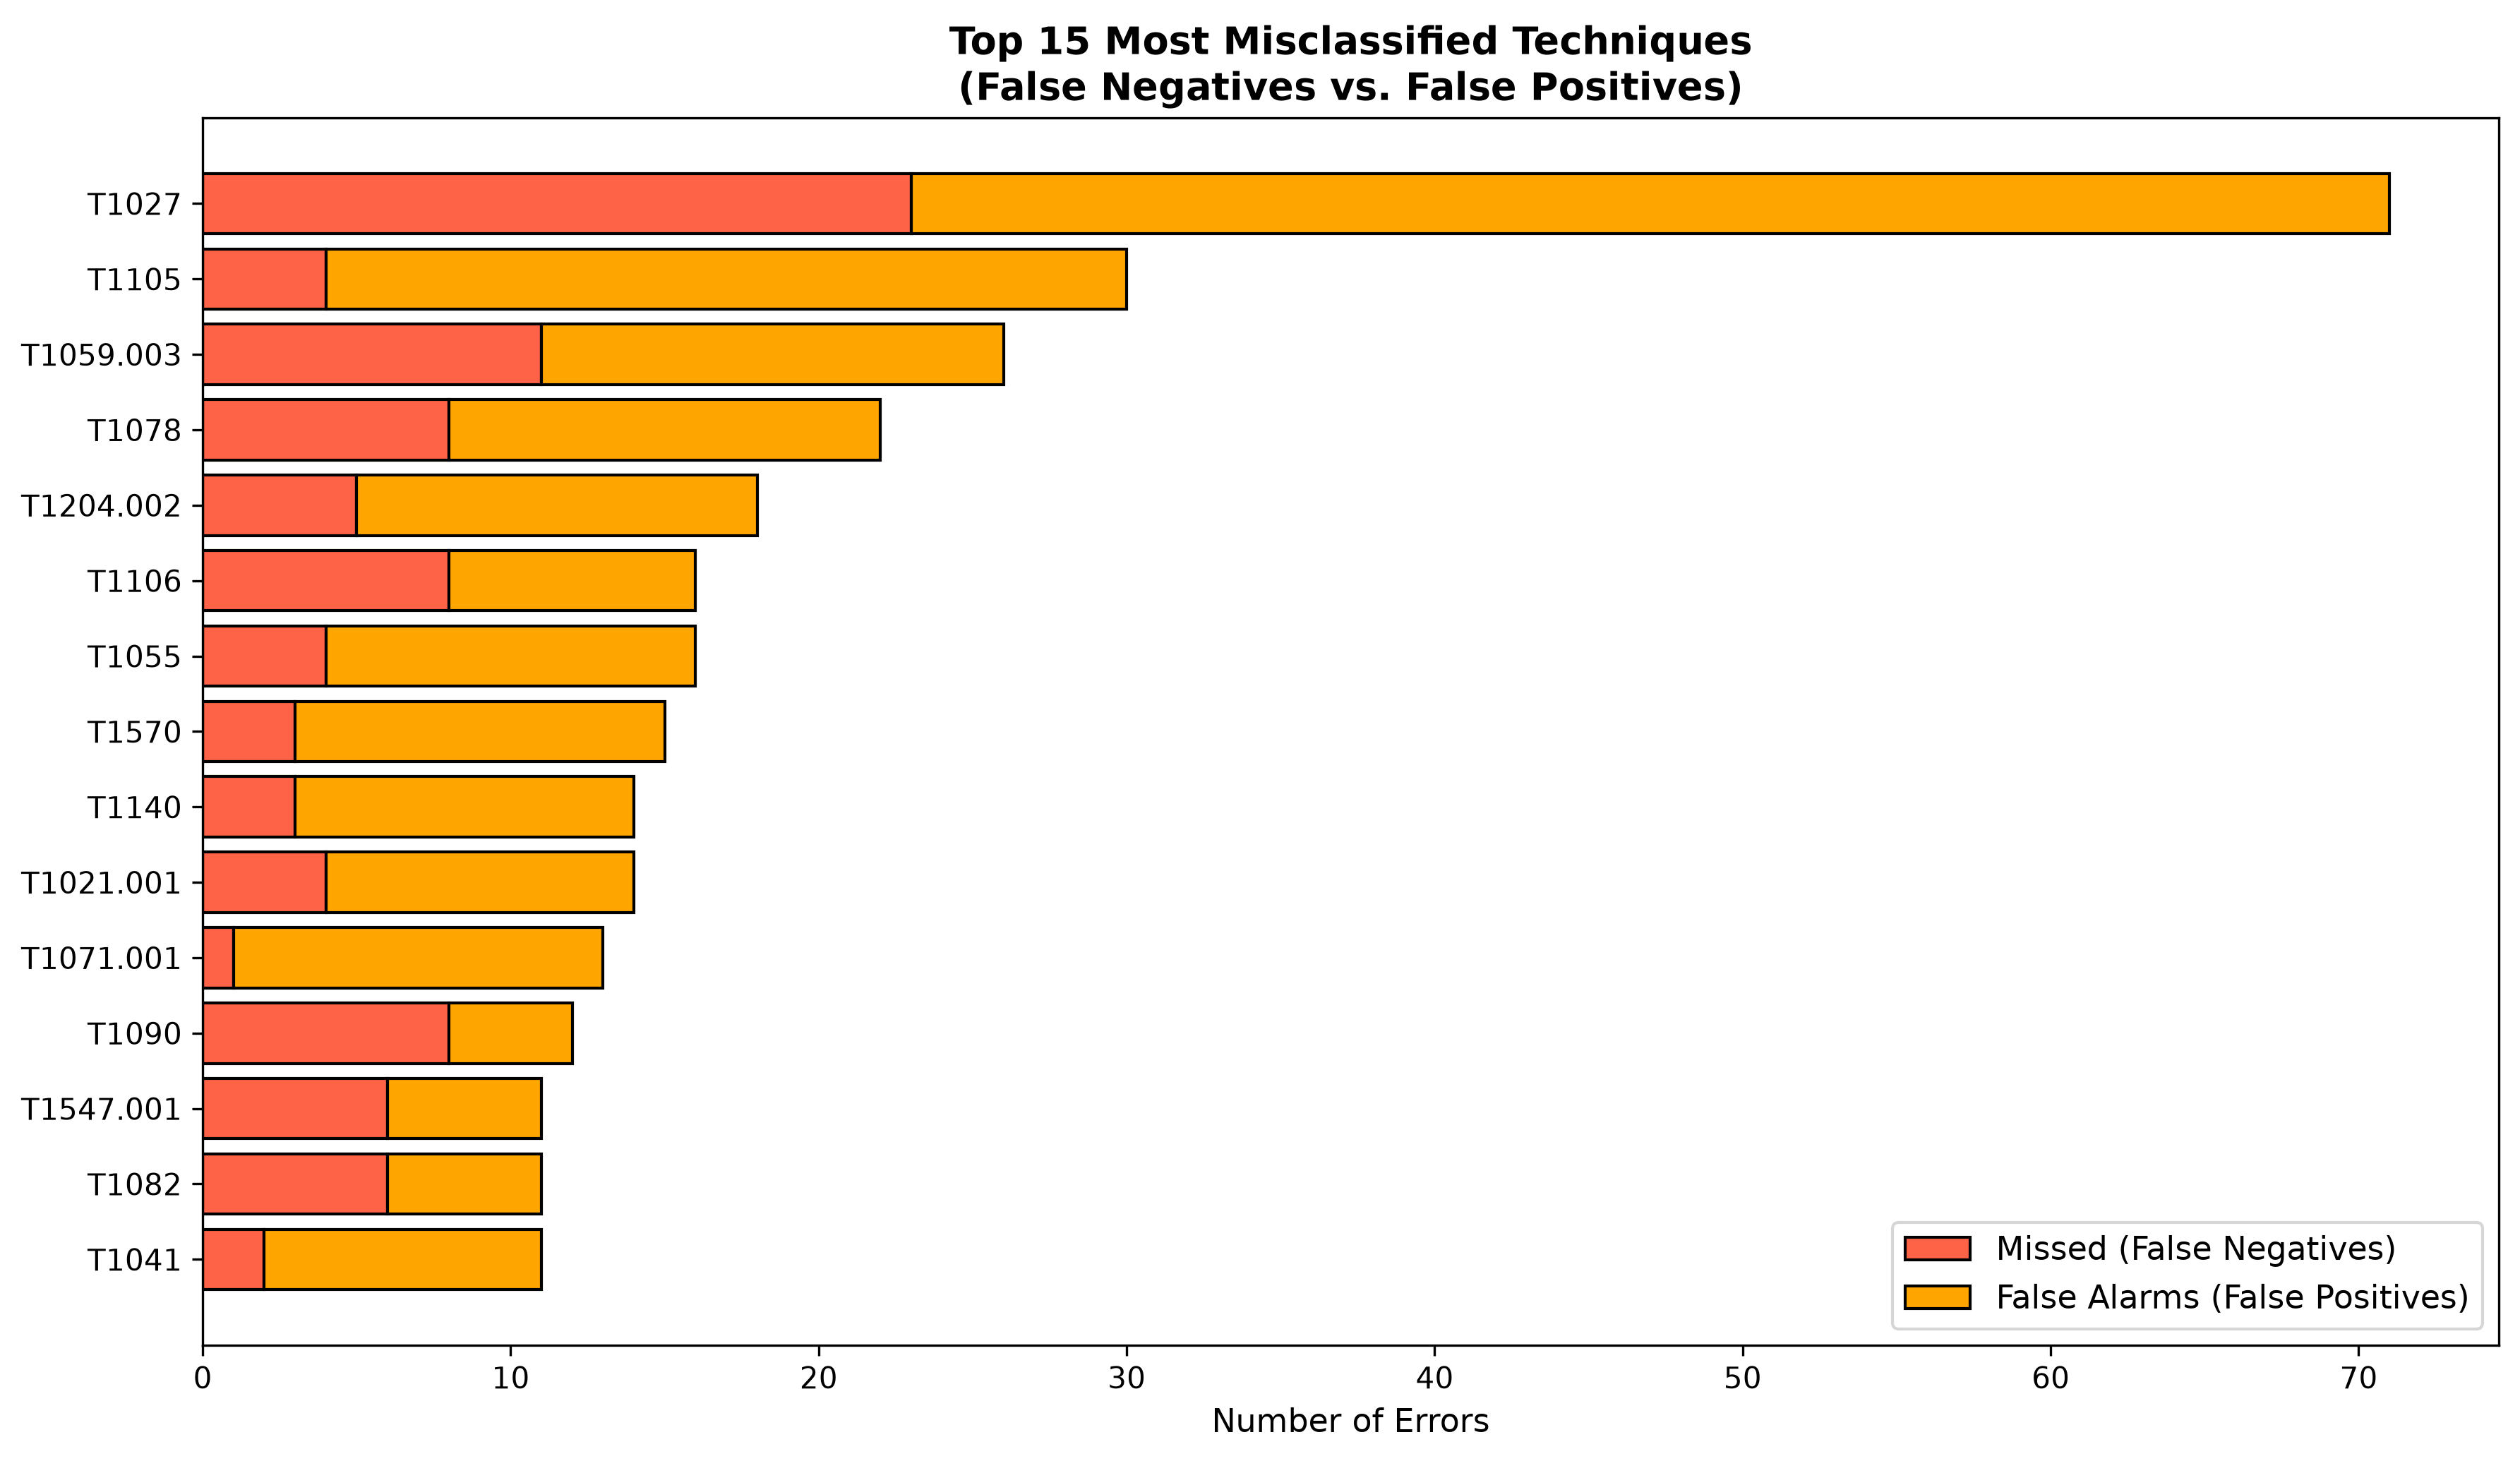
\includegraphics[width=\textwidth]{figures/tram2/tram2_cell7_plot4_error_analysis.png}
  \caption{Top-15 most misclassified techniques on TRAM~2, broken down by False Negatives (missed detections, red) and False Positives (false alarms, orange).}
  \label{fig:tram2_errors}
\end{figure}

\subsection{rcATT: Truncation-Driven Failure Modes}
On rcATT, the top-15 misclassified techniques exhibit high False Positive counts (~161 FP out of 167 test samples; Figure~\ref{fig:rcatt_errors}). Under a calibrated multi-label decision threshold ($\tau=0.35$) applied to truncated 256-token representations, the model struggles to differentiate presence from absence on long documents, highlighting that sliding-window chunking or long-context architectures are imperative for document-level threat classification.

\begin{figure}[t]
  \centering
  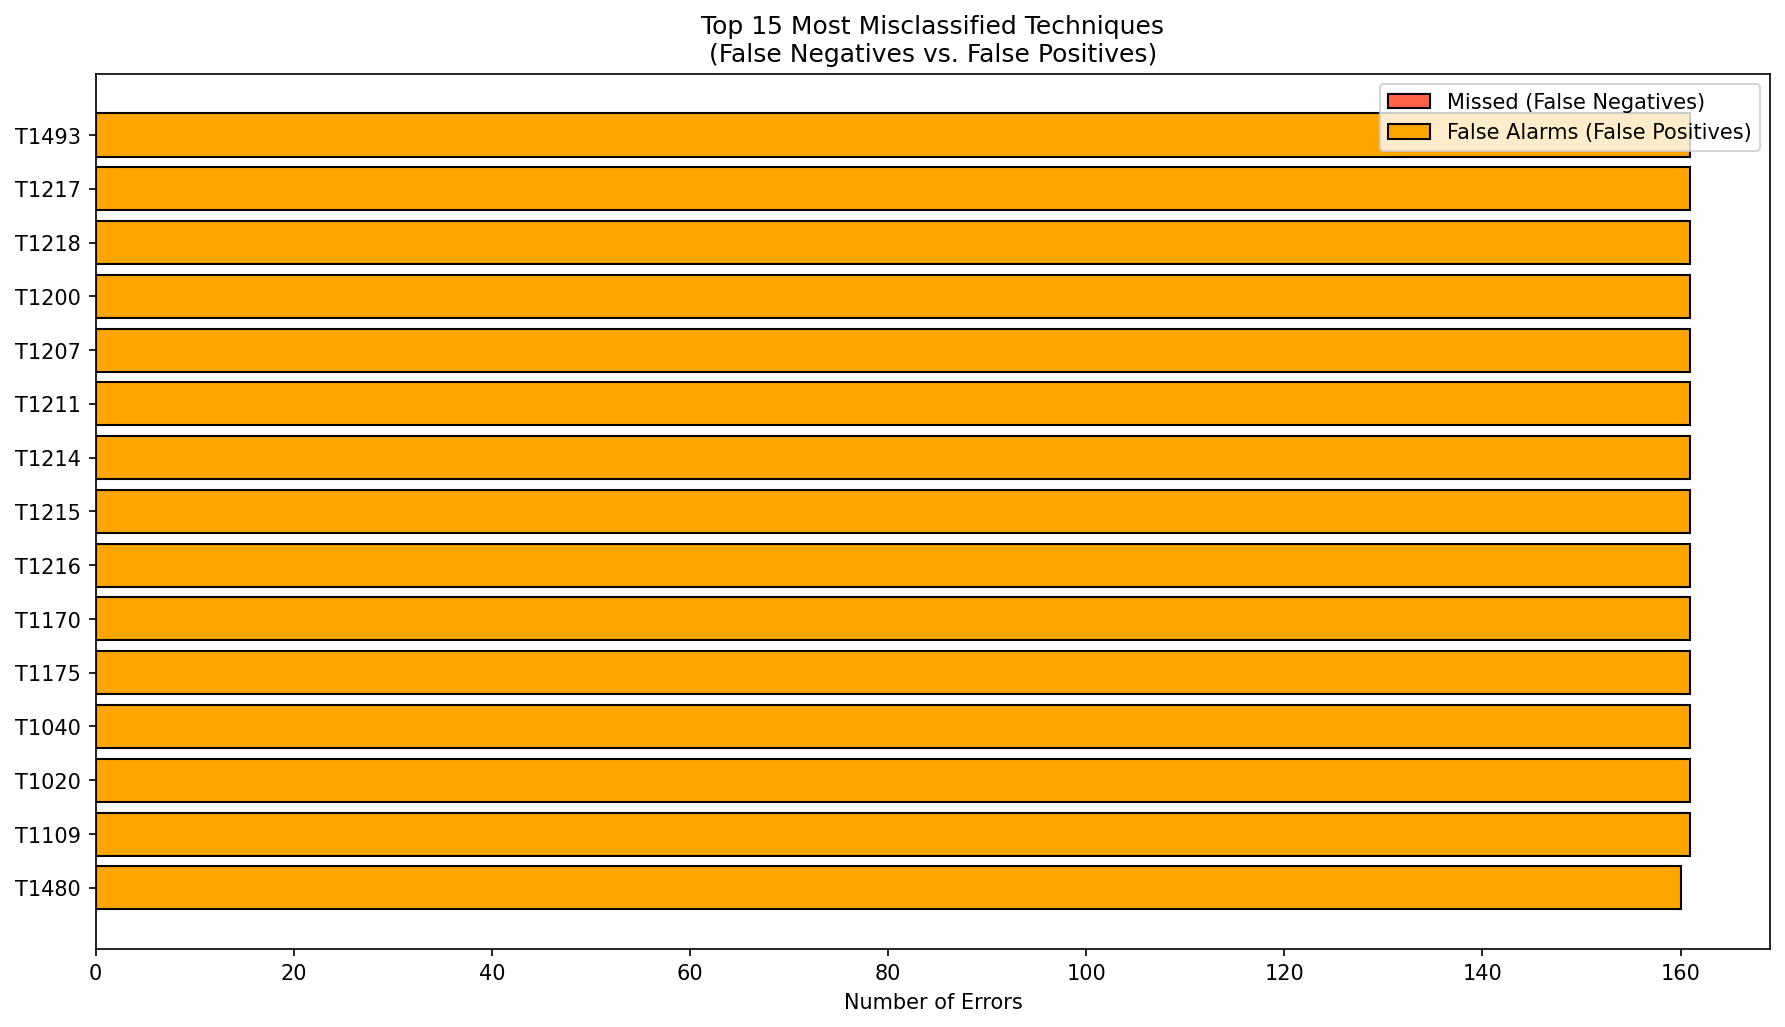
\includegraphics[width=0.85\textwidth]{figures/rcATT/rcATT_cell7_plot4_error_analysis.png}
  \caption{Top-15 techniques by error count on rcATT, dominated by False Positives due to evaluating 256-token truncated sequences under multi-label thresholding.}
  \label{fig:rcatt_errors}
\end{figure}

% ============================================================
\section{Discussion and Limitations}

\textbf{Granularity Impact:} Performance stratifies sharply by annotation granularity: single-label sentence mapping achieves robust Macro-F1 (0.6160), multi-label sentence mapping requires deliberate noise downsampling and focal optimization to reach 0.4826, while document-level classification fails under fixed short-window BERT.

\textbf{CDA vs. Rule-Based Substitution:} Contextual word substitution via masked language modeling generates more syntactically and semantically plausible security phrasing than rule-based synonym swaps. However, full parametric ablation isolating CDA from downsampling across varied threshold ranges remains an important direction for follow-up studies.

\textbf{Document-Level Scaling:} Future research on rcATT must employ sparse-attention architectures such as Longformer~\cite{beltagy2020longformer} or hierarchical chunk-pooling to preserve complete narrative chains across several thousand tokens.

% ============================================================
\section{Conclusion}

This paper presented a unified framework for automated MITRE ATT\&CK classification across three benchmark corpora. On sentence-level single-label data (TRAM~1), class-weighted cross-entropy achieves a Macro-F1 score of 0.6160. On multi-label sentences with heavy background noise (TRAM~2), coupling 1:1 downsampling, Contextual Data Augmentation, and Focal Loss yields a +74.5\% relative Macro-F1 gain (to 0.4826) with an Exact Match Ratio of 0.6130 and consistent stability across repeated trials. On full reports (rcATT), we empirically confirm that fixed 256-token encoders retain only 3.9\% of document content, resulting in severe truncation failure. Cross-benchmark error analysis establishes T1027 obfuscation vocabulary overlap as the primary failure mode, defining a clear roadmap for future context-aware threat intelligence systems.

\section*{Code and Data Availability}
To facilitate reproducibility while adhering to double-blind peer review requirements, experimental code, trained model checkpoints, and configuration logs will be published via an open-access repository upon acceptance.

\bibliographystyle{splncs04}
\bibliography{references}

\end{document}
